\chapter{Temporal Data Mining for Temporal Property
Detection}\label{chap:templog}

In this chapter we introduce a temporal logic based upon sequences
with NDs, possibly representing time series functions, for temporal data
mining purposes. We show how temporal properties may be formalised
within this logic and used for temporal data mining.
\smallskip

In Section~\ref{sec:tl_intro} we introduce and motivate this
work, stating why we focus on NDs. Section~\ref{sec:tl_why} follows
with a discussion of why
properties are useful for temporal data mining, concentrating on the
ability to succinctly characterise temporal behaviour. In
Section~\ref{sec:tl_nd} we briefly present NDs in a temporal database
and follow this in Section~\ref{sec:tl_tsa} with a presentation of
time series analysis. We provide this for two reasons. Principally
because our logic uses some time series analysis functions and
secondly as a comparison between our work and a standard time series
analysis that may be performed on a temporal database, noting that the
branching factors of an ND
in a temporal database may be viewed as a time series. In the next
chapter we shall see some results from applying our logic for temporal
property discovery just to time series.  Section~\ref{sec:tl_relations}
provides an introduction to temporal sequences upon which our logic is
based. In Section~\ref{sec:tl_ndltl} we formally define our temporal
logic. Finally, in Section~\ref{sec:tl_properties} we define some temporal
properties and discuss the intuition behind attempting to discover
these properties from a temporal database. \cite{jmw96} state that,
``the task of data mining can be seen as the problem of extracting the
interesting part of the logical theory of a model.'' We consider
specific properties to represent interesting patterns within our logic.
We conclude with a
discussion of the open problems that remain in~\ref{sec:tl_disc}.

\section{Introduction}\label{sec:tl_intro}
\index{snapshot!relation}
In Temporal Databases we
may view each state at time point $t$ as a snapshot of the database. 
Over a series of time points, taken at fixed intervals, each snapshot 
may satisfy changing
ND sets which may model temporal relationships previously unknown to
the database user. We assume the time intervals are fixed for clarity
within the discovery process though it would be feasible to {\em unfold}
time points over different size intervals into a fixed representation.

\smallskip

The sets of points satisfied by the ND sets across time form a time
series. We introduce in Section~\ref{sec:tl_ndltl} a temporal logic of
sequences to model aspects of
time series statistics and present them as ``properties'' of the
temporal database. The modal operators are extended from the temporal
logic operators of safety, implying at all future points, and
guarantee, implying at some point in the future, to implying all
subsequences of size $n$ and some subsequence of size $n$, respectively.  
In this way we use these operators to characterise
the temporal database with such statements as, for example, ``all
sequences of 100 days contain, at some point, a downward trend of 30
days.''  The size of the sequence may pertain to a relevant unit of
time, such as a month or a week, or length relating to behaviour of
the data in question. We also define the $\leadsto$ temporal operator which
represents a non-strict temporal ordering in that overlap is allowed.
The expression of temporal behaviour within a succinct logical
form allows for both the discovery of new knowledge and the machine
understandable form of well understood behaviour within the temporal
database. 
This has applications both in knowledge discovery and
decision support. 
\smallskip

We show how our logic may be applied to study time series for
property discovery. In Chapter~\ref{chap:tempresult} we give examples
of properties found in temporal
datasets which may be viewed as temporal relations. Loosely speaking,
properties are formulae within our language which satisfy a template
such that properties of a particular nature may be classified as, say,
conditional or persistent properties. We motivate their use in
Section~\ref{sec:tl_why}. 
We also provide
results showing interesting properties
discovered on stocks within the FTSE 100 over different
time periods. Additionally, we make use of the resampling technique
known as the {\em moving blocks bootstrap}. From an input time series we
randomly sample blocks, or in this case sequences of a size $n$, and
append the sequences to the resampled series as they are selected
until we have a resampled series of equivalent length to the original
series.  
The resampling destroys long term relationships whilst preserving
relationships of a size less than $n$, allowing us to
look for short range properties which may hold in various time series.
We apply our property discovery
algorithms to these and the original sequences and provide examples of
interesting,
useful and previously unknown properties which hold, satisfying all of
the criteria for successful knowledge discovery. We do however stress
that properties discovered may 
require expert examination for validation as a contribution to
knowledge. This is a key point for all knowledge discovery systems
\cite{fps96,man97}. We conclude in
Section~\ref{sec:tl_disc} with a
discussion proposing the inclusion of these techniques into DBMS.

\section{Why do we need properties for Temporal Data Mining?}\label{sec:tl_why}
\index{Rule Discovery}
\index{Events}
\index{Temporal Logic Properties}
\index{Properties|see{Temporal Logic Properties}}

There has been much work on properties holding in temporal logic, upon
which the seeds of this work lie, most notably \cite{mp92}. Properties
in temporal logic have arisen out of the application of temporal logic
to computing. Transition rules in a program allow for properties to be
specified. For example, the standard notation would use $\Box p \to
\Diamond q$ to denote that at all future points $p$ holds ($\Box p$)
which implies
that at some point in the future $q$ holds ($\Diamond q$) and this is
referred to as a
{\em response to insistence} property. We redefine connectives and
properties in
our logic so that we may discover various forms of response and
persistence rules for temporal sequences. We define a response rule as
\resp{n}{m} $\sigma$ which implies that all subsequences
of size $n$ ($\bm^n$) contain a sequence of size $m$ (\diam$^m$) which
satisfies $\sigma$, and a persistence rule as \pers{n}{m} $\sigma$  
stating that for a sequence of size $n$ all of its $m$ length subsequences
satisfy $\sigma$, where $m \le n$.
The contribution of this work is the use of property discovery in a
temporal logic relating to subsequences for discovering relationships
about NDs, the atoms of our logic, in temporal databases.
	
\section{Numerical Dependencies in a Temporal Database}\label{sec:tl_nd}
\index{Numerical Dependencies!in a Temporal Database}
In a Temporal Database each snapshot at a particular time may satisfy
a set of NDs. We assume that the ND set is specified via an attribute
set template provided by the database user, though we note that it is
possible to ``mine'' the relation for NDs blindly as detailed in Section~\ref{sec:nd_datamine}.

\subsection{Temporal Relation Sequences}\label{sec:tl_relations}
\index{Temporal Sequences}
\index{Sequences|see{Temporal Sequences}}


\begin{definition}[Temporal Relation Sequence]
\begin{rm}
A {\em relation sequence} (temporal database) $\Delta$ over R is a
finite set of 
relations over R with $\Delta$ = $\{ r_0, r_1, \ldots, r_n \}$,
indexed chronologically $0, 1, \ldots, n$ from an initial point 0 and
having a final point $n$, each state corresponding to a time point a
fixed interval apart from its previous and next value. $\quad\Box$
\end{rm}
\end{definition}

We assume that our relation sequence, equivalent to a temporal
database, is a collection of
relations which are linearly ordered. As such we infer within our
logic that time itself is linearly-ordered. At each moment there is
only one possible future moment. 
Our underlying sequence is finite. This is natural given that the
input for the
data mining procedures is a finite sequence of relations.


\subsection{Time Series Analysis and Numerical
Dependencies}\label{subsec:tl_tsa_nd}
\index{Numerical Dependencies!and Time Series Analysis}

We now briefly present the relationship between time series and NDs.

\smallskip

The simple example in tables~\ref{tab:1} and~\ref{tab:2} for
a relation $COLLEGE(C,S,T)$ over two years where $C$, $S$, and $T$
represent course, student and tutor, respectively, highlights possible
transition in a temporal database. The change in ND set satisfaction
for the ND set = $\{ C \to^k S, C \to^k T \}$ from $\{ C \to^3 S, C \to^2 T \}$
to $\{ C \to^4 S, C \to^1 T \}$ may be an indicator of both increasing
student numbers on courses whilst at the same time implying that
tutors have more work to do on a course. This information could be
represented in a single relation if timestamps were attached to each
tuple.

{\line
\begin{table}[ht]
\begin{minipage}[b]{7.2cm}
\begin{center}
\begin{tabular}{|c|c|c|} \hline
 C & S & T \\ \hline
 b11a & Paul & Mark \\ 
 b11a & Tina & Mark \\
 b11a & Fred & Robin \\
 b151 & Paul & Robin \\ \hline
\end{tabular}
\end{center}
\caption{\label{tab:1} 1997 student intake records}
\end{minipage}
\hfill
\begin{minipage}[b]{7.2cm}
\begin{center}
\begin{tabular}{|c|c|c|} \hline
 C & S & T \\ \hline
 b11a & Tom & Mark \\
 b11a & Dan & Mark \\
 b11a & Louise & Mark \\
 b11a & Jim & Mark \\
 b151 & Jim & Robin \\ 
 b151 & Jose & Robin \\ \hline
\end{tabular}
\end{center}
\caption{\label{tab:2} 1998 student intake records}
\end{minipage}
\end{table}
}


Clearly, the change in ND set satisfaction may be viewed as a
time series. For example, $C \to^{16} S$, $C \to^{20} S$, $C \to^{27} S$ may
be viewed as a time series of points $16,20,27$ assuming a fixed time
interval between insertion.

\medskip

The requirement that for a template of NDs provided for a relation the
ND set only changes on the branching factor may be seen as
restricting. Schema evolution \cite{oe92,rod94} may remove an attribute from
the relation thereby making an ND in a given set null and void. We
assume the following: (1) For the input provided the schema is fixed,
and (2) changes in the schema can be assessed by separate mining
processes on two separate relation sequences, one before and the other after
any schema update.  


\section{Time Series Analysis}\label{sec:tl_tsa}
\index{Time Series Analysis}
We now provide a brief overview of time series analysis. In
Section~\ref{subsec:tl_tsabasic} we discuss research on time series
analysis and emphasise areas which our work may be considered as
contributory to. Then in Section~\ref{subsec:tl_tsadefs} we provide
definitions of standard functions used within linear time series
analysis which are embedded within our logic.

\subsection{Time Series Analysis: Basics}\label{subsec:tl_tsabasic}

The goal of time series analysis is to model an observed system so
that its future behaviour may be predicted \cite{wg94}. We discuss
both traditional time series analysis and new techniques, such as the
use of neural networks, and then relate this to our work. Having read
this section the reader will fully appreciate the statistical
functionality we incorporate into our logic, presented in
Section~\ref{sec:tl_ndltl}. We assume familiarity with the statistical
functions, such as variance, covariance, correlation, autocorrelation
etc, defined in Section~\ref{subsec:tl_tsadefs}.

\medskip

The standard methodology for analysing a time series is to decompose
the series into trend, seasonal and irregular components, each of
which may be expressed as individual functions of time. \cite{wg94}
demarcates the difference between understanding and learning from a
time series as that of applying explicit mathematical insight for
model creation to that of using
learning algorithms to emulate the behaviour of the time series. Our
goal is closer in spirit to understanding the sequence, using
properties to achieve this. For linear and stationary time series one
of the most popular techniques is to create an autoregressive (AR) model,
of the following form for the Mth order AR model, where the first $M$
autocorrelations determine the coefficients \cite{end95}:
\begin{displaymath}
x_t = \sum_{m=1}^M a_m x_{t-m} + e_t
\end{displaymath}
where $e_t$ represents noise and $a_m$ the autoregressive
coefficients for $x_t$ on $x_{t-1}$, $x_{t-2}$, $\ldots$, $x_{t-M}$; $e_t$
is assumed to have expectation 0 and is independent of previous
values. Moving Average (MA) models can also be characterised by
autocorrelation coefficients describing how values $\tau$ steps apart
co-vary with each other. \cite{ko90} remark that autocorrelation
coefficients for large lags are unreliable for model
identification. We found this to be true within our logical
representation and adopted their advice of restricting lags of a time
series with $n$ points to lags up to $\frac{n}{4}$. This seemed to be
a sensible 
restriction across all time series sizes, given that the reliability
of the lag values decrease for higher lags and that we are using
sequences of a size chosen by the user which may be arbitrarily short.

\medskip

AR and MA models may themselves be combined to form ARIMA models,
denoting Autoregressive Integrated Moving Average models, integrated
implying that we are dealing with a stationary time series, after {\em
differencing}.
We omit a full discussion of model selection,
provided in
\cite{ko90,end95}, suffice to say that ARIMA models have had the
greatest impact on linear time series analysis. Other aspects of time
series analysis are the Yule-Walker equations which allow the
autocorrelation coefficients of a time series to be expressed by
autoregressive coefficients. This is simply understood given their
definitions; see \cite{ko90}. The restriction of analysis methods to
linear time series may cause problems. Two approaches to combat this
are:
\begin{enumerate}
\item Approximating a system with more than one linear model, known as
local linear modelling. \cite{wg94} state that many regions must be
selected if the nonlinearity is of a quadratic degree or greater.
\item The use of differencing to remove trend. \cite{naze88,end95}
comment that most nonstationary time series, where nonstationary
implies a trend, can be changed to
stationary time series by differencing once or twice. Given a series
\series{n} we obtain the first and second order differenced series by 
$y_2 - y_1, y_3 - y_2, \ldots, y_n - y_{n-1}$ and 
$y_3 - 2y_2 + y_1, y_4 - 2y_3 + y_2, \ldots, y_n - 2y_{n-1} +
y_{n-2}$, respectively. \cite{naze88} comments that most economic time
series are stationary after at most second order
differencing. \cite{raf99} refers to differencing as {\em momentum}.
\end{enumerate}

Our logic incorporates aspects of local linear modelling by breaking a
time series into sequences which may then be linearly regressed within
the sequence; we also allow differencing within our
logic. \cite{naze88} states that ``the best practical approach in
examining a series is visual examination of the plot of the series.''
It is a key intention of this work to provide a definite contribution
to any visual examination of a time series.  

\medskip

Nonlinear time series have most recently been the subject of analysis
by neural networks. \cite{wg94} stresses the importance of
differentiating between learning for model discovery and simple
memorisation. The latter occurs when the data is overfitted and
prediction relies too heavily on previous values (including noise)
rather than looking for a model. The complexities of non-linear time
series analysis are outside the remit of this work. We believe that
the application of sequences to differenced, and/or moving averaged,
time series implies that our
procedures can still obtain meaningful properties from such non-linear series.
This is due to the fact that though there may not be any global linear
properties 
of the time series our use of sequences breaks the time series up and
within these sequences there may be linear behaviour allowing for
potentially interesting knowledge discovery. \cite{cl96b} notes some
strengths of local regression stating it adapts well to high
curvature, can be tailored for many distributional assumptions, and is
easy to understand and implement.

\subsection{Time Series Analysis: Definitions}\label{subsec:tl_tsadefs}
\index{Time Series Analysis!Definitions}

We now present the standard statistical functions used within linear
time series analysis \cite{ko90}.
\index{variance!of a time series}
\begin{definition}[Variance]\label{def:var}
\begin{rm}
Given a time series $x$ of length $n$, its variance is written as
$var(x)$ where
\[
var(x) = \frac{1}{n-1} \sum_i^n (x_i - \mu)^2
\]
We assume that the series is stationary having a mean value $\mu$.$\quad\Box$
\end{rm}
\end{definition}

\index{standard deviation!of a time series}
\begin{definition}[Standard Deviation]\label{def:sd}
\begin{rm}
Given a time series $x$ its standard deviation is $\sigma_x$ where 
\[
\sigma_x = \sqrt{var(x)}\quad\quad\Box
\]
\end{rm}
\end{definition}
\index{covariance}
\begin{definition}[Covariance]\label{def:covar}
\begin{rm}
Given two time series $x$ and $y$, both of length $n$, their
covariance is written as $cov(x,y)$, where
\[
cov(x,y) = \frac{1}{n} \sum_i^n (x_i - \mu_x) (y_i - \mu_y)
\]
We assume that the series $x$ and $y$ are stationary with mean values
$\mu_x$ and $\mu_y$, respectively.$\quad\Box$
\end{rm}
\end{definition}

Covariance is a measure of the linear association between two variables.
The strength of the relationship unfortunately depends on the unit of
measurement used and so to avoid this we introduce the correlation
coefficient.
\index{correlation coefficient}
\begin{definition}[Correlation Coefficient]\label{def:correl}
\begin{rm}
Given two time series $x$ and $y$ the correlation coefficient
$cor(x,y)$ is
\[
cor(x,y) = \frac{cov(x,y)}{\sigma_x \sigma_y}\quad\quad\Box
\]
\end{rm}
\end{definition}

The regression coefficient determines the slope for a series of values
where $y$ is time when dealing with temporal sequences.
\index{regression coefficient}
\begin{definition}[Regression Coefficient]\label{def:regcoef}
\begin{rm}
Given a time series $x$, the regression coefficient
$reg(x)$ is
\[
reg(x) = \frac{cov(x,y)}{\sigma_y}
\]
where $y$ represents time.$\quad\Box$
\end{rm}
\end{definition}

We note that regression is equivalent to correlation but without
the standard deviation of $x$ in the denominator. Therefore, unlike
regression, 
correlation does not make a distinction between the $y$-value and the
value upon which it is regressed, in our case time. Another process
for determining the trend of a sequence is to use discordance which
sums the value comparisons over all possible pairs of values to
determine trend, defined as: 
 
\index{discordance}
\begin{definition}[Discordance Test]\label{def:disccoef}
\begin{rm}
Given a time series $y$ = $\{$ \series{n} $\}$, we let
\begin{eqnarray*}
q_{ij} & = & 1, \quad\mbox{if}\quad y_i > y_j \quad\mbox{when}\quad j > i \\
       & = & 0, \quad\mbox{otherwise}
\end{eqnarray*}
We define $Q$ as:
\[
Q = \sum \sum_{\!\!\!\!\!\!\!\!\!\!\!i < j} q_{ij}
\]

Now, this series is random under the null hypothesis and since there
are $n$ points in the time series then there are $\frac{1}{2} n(n-1)$
pairs and so the expected value of $Q$, E($Q$) = $\frac{1}{4} n(n-1)$
Our discordance function for a time series $y$ is:
\begin{eqnarray*}
discord(y) & = & 1,  \quad Q < E(Q) \\
      	   & = & -1, \quad Q > E(Q) \\
	   & = & 0,  \quad \mbox{otherwise} \quad\quad\Box
\end{eqnarray*}
\end{rm}
\end{definition}

Autocovariance and autocorrelation are presented as we may wish to
compare sequences of the same time series.
\index{autocovariance}
\begin{definition}[Autocovariance]\label{def:autocovar}
\begin{rm}
Given a time series $x$, of length $n$, its autocovariance of lag $k$
(or lead $-k$) is written as $autocov(x,k)$ where
\[
autocov(x,k) = \frac{1}{m} \sum_i^m (x_i - \mu_x) (x_{i-k} -
\mu_{x})\quad\mbox{where}\quad m = n-k 
\]
We assume that the series $x$ is stationary with mean value
$\mu_x$.$\quad\Box$ 
\end{rm}
\end{definition}

\index{autocorrelation coefficient}
\begin{definition}[Autocorrelation Coefficient]\label{def:autocorrel}
\begin{rm}
Given a time series $x$ the correlation coefficient $acor(x,k)$ is
\[
acor(x,k) = \frac{autocov(x,k)}{\sqrt{var(x)var(x-k)}}\quad\quad\Box
\]
\end{rm}
\end{definition}

\index{cross covariance}
\begin{definition}[Cross Covariance]\label{def:crosscovar}
\begin{rm}
Given two time series $x$ and $y$, both of length $n$, their
cross covariance of lag $k$
(or lead $-k$) is written as $ccov(x,y,k)$ where
\[
ccov(x,y,k) = \frac{1}{n} \sum_i^n (x_i - \mu_x) (y_{i-k} - \mu_y)
\]
We assume that the series $x$ and $y$ are stationary with mean values
$\mu_x$ and $\mu_y$, respectively.$\quad\Box$
\end{rm}
\end{definition}
 
\index{cross correlation coefficient}
\begin{definition}[Cross Correlation Coefficient]\label{def:crosscorrel}
\begin{rm}
Given two time series $x$ and $y$ the cross correlation coefficient $ccor(x,y,k)
$ is
\[
ccor(x,y,k) = \frac{ccov(x,y,k)}{\sigma_x \sigma_y}\quad\quad\Box
\]
\end{rm}
\end{definition}

\subsection{Catalytic Data Mining}\label{subsec:tl_catdm}
\index{Catalytic Relation|see{Catalytic Data Mining}}
\index{Catalytic Data Mining}

Catalytic Data Mining is a term introduced by \cite{HS95} for the data
mining of two or more relations which agree on a common attribute or
more so that the data mining process can be enhanced. We mention it
here given that it applies to NDs in temporal relations. Our data
mining process is such that for a company we can extract NDs from
either an employee or product sales relation and 
then perform the mining on this together with a directly numerical
value such as the stock price. Over time a fall in stock price
combined with little change in an ND in the sales relation each
October may suggest that a sale is held at this time of year to
increase sales.

\subsection{Advantages of a logical approach}
\index{Linear Temporal Logic|see{Numerical Dependency LTL}}
\index{Temporal Logic}
\index{Modal Logic!see{Temporal Logic}}

Standard time series techniques allow us to apply time series functions
to time series naively. This, in turn, may produce useful results such
as a high cross-correlation between two time series. A symbolic
representation of this provides similar information without recourse
to numerical comparison. Therefore our logic is algorithmic and
as such is amenable to symbolic manipulation. This implies that it is
of use within decision support tools and perhaps general data mining
systems.

\medskip

The logic is also flexible so that many
different kinds of relationships and patterns can be expressed in a
very concise form. This is a result of using a high-level logic to
represent desired concepts. 


\section{Numerical Dependency Linear Temporal Logic}\label{sec:tl_ndltl}
\index{Numerical Dependency LTL}

We now formalise our temporal logic for sequences which we refer to
henceforth as NDLTL. Much of the intuition behind sequences follows
from Allen's temporal intervals which we advise reading for a clear
understanding of the use of intervals and sequences in time
\cite{all84}.

\subsection{Temporal Logic}
\index{Temporal Logic}
Propositional Linear Temporal Logic is propositional logic augmented
with the modalities ${\cal S}$ and ${\cal U}$, denoting since and
until, respectively, defined in \cite{ghr94}. For atoms A and B, A ${\cal S}$ B is true at time $t_n$,
if for time $t_0$ where $t_0 < t_n$, if B is true at $t_0$ and for all
points between $t_0$ and $t_n$, A is true. Similarly, A ${\cal U}$ B
is true at $t_p$ if for some $t_q$ where $q > p$, B is true at $t_q$
and for all points between $t_p$ and $t_q$, A is true. 
From these modal primitives further temporal
operators may be defined, of which the principal ones are $\Box$ and
$\Diamond$, implying, respectively, at all future points and at some
point in the future. 
$\Diamond$ A may be defined as {\em true} ${\cal U}$ A, $\Box A$ is the dual
of $\Diamond$ A defined as $\neg \Diamond \neg$ A.  $\bigcirc$ A,
representing {\em nexttime} A, may be defined as {\em false} ${\cal U}$ A
\medskip

A logic may be created due to concerns that there are inadequacies
within previous logics to represent various kinds of informal argument
\cite{haa78}. We wish to represent arguments representing aspects of
time series analysis within a logical form that allows patterns in the
temporal sequences to be represented; a logic is a system for
obtaining answers from $\Delta$ \cite{ghr94}. Our logic is with respect to
sequences of temporal relations, equivalent to the interval
representation of time \cite{all84}.
We modified our logic to contain $\leadsto$ and $\bm^n$ as primitives
with respect to sequences. Formulae of the form $\sigma_1 \leadsto
\sigma_2$ imply that a sequence $s_1$ starts before $s_2$ and
ends before $s_2$ ends, with $s_1$ satisfying $\sigma_1$ and $s_2$
satisfying $\sigma_2$. If a sequence $s_1$ satisfies $\bm^n \sigma$
this implies that all sequences of size $n$ in $s_1$ satisfy
$\sigma$. 

\medskip

Another possible approach would have been to incorporate the time
series operators at the atomic level and apply these within a standard
temporal logic for knowledge discovery. We now show by example some
potential problems with this. A sequence $s$ may satisfy
ccor($\sigma_1$, $\sigma_2$, $k_1$) ${\cal U}$ ccor($\sigma_1$,
$\sigma_2$, $k_2$). Even if we allow the inclusion of such time series
functions we are likely to discover that time series are unlikely to
satisfy a formulae A ${\cal U}$ B without numerous conjuncts leading
to formulae such as A ${\cal U}$ B ${\cal U}$ C ${\cal U}$ A ${\cal U}$
B. The problem with using standard {\em point based} temporal logic
for the discovery of 
such formulae is that they are apt to {\em overfit} the data; in this 
brief example we have A ${\cal U}$ B holding twice. It would be of
more value to be able to represent this fact, which our logic of
sequences achieves in some respect. Standard temporal logic models
atoms occurring at certain time points such as inferring A ${\cal U}$ B over
a period of $p$ time points. This, within a point based
logic, may lead to the discovery of many hundreds of
formula. However, we approach our discovery from the
basis of creating sequences so that we control the granularity of 
property discovery given that we may have to
deal with many hundreds of time points.  Though this may result in
valuable knowledge found we 
believe a sequence based logic results in finding {\em interesting}
knowledge more easily.
Similarly
$\Box A$, denoting at all points in the future A holds in temporal
logic, is unlikely to 
either be satisfied or, if it does, represent interesting
information. Another potential problem is that the discovery of
temporal logic formulae without restriction may often be too complex for
efficient knowledge discovery; formulae such as (C ${\cal U}$ A)
${\cal S}$ (B ${\cal U}$ C) or $\Box$ (A $\to$ $\Diamond$ D). These
formulae themselves do not represent complex behaviour, for example,
the former proposition may hold if C occurs between one or more
occurrence of both B and A. Therefore we choose to
restrict our discovery to search for what we believe are interesting
formulae.
\medskip

These
deficiencies suggest that formulae be verified with respect to
sequences. Therefore, we have modified our modal operators with
respect to sequences. We also introduce $\leadsto$; this is a temporal
ordering operator which allows overlap. We motivate its inclusion
based on the fact that within time series and temporal sequences
strict transitions of properties may not occur. The formalisation of
$\leadsto$ is sufficiently flexible yet restrictive enough to discover
interesting patterns within and across sequences. The requirements
outlined in \cite{ghr94} for the components for specification of a
temporal logic are all provided in our formal definition apart from
allowing our units of time to vary across data sets, though we may
generalise and say that time is the set of integers, satisfied in all
data sets. 

\smallskip

We shall demonstrate, informally, how sequence-based temporal operators
are more appropriate for data mining applications. As we shall see in
section~\ref{subsec:logic_query} our discovery process is
computationally efficient due to our restriction of fixed sequence
sizes which allow for polynomial time knowledge discovery. We assume that we
have as input a finite temporal database; given this it is of minimal
value to search for certain temporal logic formulae. The discovery of
$\Diamond \sigma$ in state $i$, say, tells us little in a knowledge
discovery sense.  Additionally, the random discovery of useful formula
is a challenging task given that there may be a significant number of
different patterns within a temporal database. The division of an
input sequence into all possible sequences of a size chosen by the
user allows knowledge discovery over all possible different time
periods within the input sequence. Sentences not containing any of the
sequence or temporal operators reduce to sentences of classical
propositional logic with NDs and ND time series functions as atoms.

\medskip

Our logic has additional operators which incorporate a means of
representation for time series analysis techniques within our
logic. Therefore our logic allows information about the input data to
be analysed with respect to a given time period specified by the user
within which techniques such as regression and correlation are applied
and then the rules for the time periods themselves are analysed for
possible properties which may hold in a sequence. The complexity of
temporal logic and time series implies that it is highly unlikely that
we will discover a rule of the form $\Box \sigma$ at a particular
point, unless the input is near trivial in which case it is
uninteresting. Similarly, $\Diamond \sigma$ is uninteresting due to
its general application.

\medskip

The modal operator $\bm^n$ is not, in the strict sense, a temporal
operator. A system is considered temporal if it has an (irreflexive
transitive) ordering $<$ \cite{ghr94}. Our operator $\bm$ makes use of
inclusion (of sequences), see Definition~\ref{tl_def:inclusion}, which
refers to set containment as opposed to ordering.

\smallskip

We remark that our logic is non-monotonic in that properties
discovered for a sequence may not hold if we apply the same discovery
algorithms to an updated version of the same sequence, containing a
longer sequence. As such fewer properties are likely to hold
demonstrating the non-monotonicity of this approach. In temporal
databases logics for integrity constraints are necessarily
monotonic, unless the semantics of the database are altered;  
this is not the case for data mining.  \cite{ghr94} notes
that monotonicity in temporal logic requires further study. 


\subsection{Syntax}
\index{Numerical Dependency LTL!Syntax}


We refer to a particular relation at state $j$ within a relation
sequence $\Delta$ as $(\Delta,r_j)$. We refer to a subsequence $s$ of
$\Delta$ ($s \preceq \Delta$) as ($\Delta$,$s$).
$r_j$ is relation at point $j$ and $r_j \models N_j$, the set of
NDs satisfied by $r_j$ and $N_j$ is an approximation to an FD set $F$
which is given as input in our discovery model.  
$\Delta$ may be omitted if the sequence is understood from the context.
We may use $\Delta \models \sigma$ to represent ($\Delta$,$\Delta$)
$\models \sigma$.

We define two operators for inclusion and ordering of sequences
referred to in the semantics of our logic, after initially defining
a sequence.

\begin{figure}
\begin{minipage}{6cm}
\centerline{\scalebox{0.7}{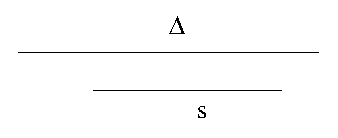
\includegraphics{templog/inclusion.eps}}}
\caption{\label{fig:inclusion} {Sequence Inclusion, $s \preceq \Delta$}}
\end{minipage}
\hfill
\begin{minipage}{6cm}
\centerline{\scalebox{0.7}{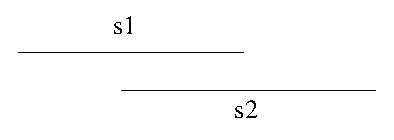
\includegraphics{templog/ordering.eps}}}
\caption{\label{fig:ordering} {Sequence Ordering, $s1 \lessdot s2$}}
\end{minipage}
\end{figure}

\begin{definition}[Sequence]\label{tl_def:sequence}
\begin{rm}
$s$ is a sequence of relations within a temporal relation sequence
$\Delta$ {\em iff} $\forall r_i \in s$ we have $\neg \exists r_l \in \Delta$ such that $r_j \le r_l \le r_k$ and
$r_j,r_k \in s$ but $r_l \not\in s$. $\quad\Box$
\end{rm}
\end{definition}

Definition~\ref{tl_def:sequence} enforces that all sequences are
continuous. 

\index{inclusion operator}
\begin{definition}[The inclusion operator, $\preceq$]\label{tl_def:inclusion}
\begin{rm}
$s \preceq \Delta$ {\em iff} $\forall r_i \in s$ we have $r_i \in \Delta$
and $s$ is a sequence in $\Delta$. $\quad\Box$
\end{rm}
\end{definition}

$s \preceq \Delta$ implies that $s$ is a subsequence of $\Delta$ and
that $s$ contains a series of consecutive states, as illustrated in~\ref{fig:inclusion}.

\index{Temporal Ordering operator}
\begin{definition}[The Temporal Ordering operators, $\lessdot$ and $\gtrdot$]
\begin{rm}
$s_1 \lessdot s_2$ {\em iff} $\quad \exists r_j \in s_1$ such that $\forall r_k
\in s_2$ we have $j < k$ and $\exists r_p \in s_2$ such that $\forall r_m
\in s_1$ we have $p > m$ and $s_1,s_2$ are sequences. $\gtrdot$ is
defined similarly. $\quad\Box$ 
\end{rm}
\end{definition}

The intuition behind our temporal ordering operator is that a sequence
comes before another sequence if at least one point in the sequence
$s_1$ is
before any in $s_2$ and $s_2$ has at least one point after $s_1$. As
desired, a subsequence of another sequence does not satisfy this
relation. Figure~\ref{fig:ordering} shows an example of sequence
ordering with an overlap between sequences.


The set of formulae of NDLTL is the
least set generated by:
\begin{enumerate}
\item Each ND $X \to^{{k}^\ast} Y$ or $X \to^{\updownarrow
{k}^\ast} Y$ is an atomic formula where ${k}^\ast \in \{ k,
\bar{{k}}, \ddot{{k}} \}$
  and $\updownarrow  \in \{ \uparrow,
\downarrow, \uparrow_r,\downarrow_r,\uparrow_d,\downarrow_d \}$.
\item If $\sigma_1$ and $\sigma_2$ are formulae then so are $\neg \sigma_1,
\sigma_1 \wedge \sigma_2, \sigma_1 \wedge^k \sigma_2$ (\mbox{k is a
constant}) and $\sigma_1 \leadsto \sigma_2$. 
\item If $\sigma$ is a formula then so are $\bm^m \sigma$ and  \diam$^m$ 
$\sigma$.
\end{enumerate}

We now define the semantics of our logic inductively.

\subsection{Semantics}\label{subsec:tl_semantics}
\index{Numerical Dependency!Semantics}
Relation state formulae are not concerned with the sequence size
used. They are obtained by performing operations on the complete
temporal relation sequence, $\Delta$. These operations represented the
ND holding at a particular state, the moving average value for a
window size $w$, or the differenced value for a particular state. We
write ($\Delta$, $u$) $\models^w$ $\sigma$ to mean that $\sigma$ holds
with respect to a window size $w$ in sequence (or state) $u$ of the
temporal relation sequence $\Delta$. We may omit $w$ if it is not
pertinent to $\sigma$; for example, $\sigma$ may be an ND alone and
$u$ may be a single relation state. The discussion of
Section~\ref{sec:tl_tsa} motivated the need for differencing. Second
order differencing, not directly expressible in our logic, is
occasionally required; an additional axiom could be added similar to
our differencing formulae.


\subsubsection{Relation State Formulae:}
\begin{enumerate}

%% STANDARD ND RULE
\item\label{item:nd} ($\Delta$, $r_j$) $\models^w$ ($X
\to^{k} Y$) { \em iff } $r_{j}$ $\models X \to^{k} Y$.

%% MOVING AVERAGE RULE
\item\label{item:ma} ($\Delta$, $r_j$) $\models^w$ ($X
\to^{\bar{{k}}} Y$) { \em iff } $r_{j-m}$
$\models X \to^{{k}_1} Y$,  $r_{j-(m-1)}$
$\models X \to^{{k}_2} Y$, $\ldots$,  $r_{j}$
$\models X \to^{{k}_{m+1}} Y$,  $r_{j+1}$ 
$\models X \to^{{k}_{m+2}} Y$, $\ldots$,  $r_{j+m}$
$\models X \to^{{k}_n} Y$ where $m = \frac{w-1}{2}$, $w$ is odd
and $\bar{{k}} = \frac{1}{w} \sum_{i = 1}^{w} {k}_i$
and $j - m \ge 0$ and $j + m \le 0$.

\item\label{item:diff} ($\Delta$, $r_j$) $\models^w$ ($X 
{\to}^{\ddot{{k}}}  Y$) { \em iff } $j > 0$ and $r_{j-1}$
$\models X \to^{{k}_1} Y$ and  $r_{j}$
$\models X \to^{{k}_2} Y$ with $\ddot{{k}} = {{k}_1} -{{k}_2}$.


\end{enumerate}

Definition 2 provides the moving average value for a {\em window} of size
$w$ for the branching
factors of the NDs for relation state $j$. At times we omit $w$ from the
following definitions for clarity. Definition 3 above provides a
difference ND values, from which a differenced sequence may be created.

All the following time
series functions used are defined in Section~\ref{subsec:tl_tsadefs}.

Relation subsequence trend formulae are required to represent trends
within our logic. These may be strict, linearly regressed, or
discordant trends. Informally, a $\uparrow$ denotes an upward trend
and $\downarrow$ a downarrow trend. We may subscript these with either
a $d$ or an $r$ to represent discordance or regression, respectively. 
In the following formulae we abbreviate {\em such that} to $s.t.$ and
denote the first relation $r_i$ in a sequence $s$ by $fst(s)$. We also
refer to a particular ND $X \to^k Y$ sequence in 
$s$ as $s_{XY}$ where necessary.

\subsubsection{Relation Subsequence Trend Formulae:}

\begin{enumerate}
%% UPWARD TREND OF MOVING AVERAGES

\item\label{item:ma_inc}($\Delta$, $s$) $\models^w$ ($X
\to^{\uparrow\bar{k}_1} Y$) { \em iff } $\mid s \mid \ge 2$ and $ \forall r_{j},r_{j+1} \in
s$ ($\Delta$, $r_j$) 
$\models^w X \to^{\bar{k}_1} Y$ and ($\Delta$, $r_{j+1}$) 
$\models^w X \to^{\bar{k}_2} Y$ for some $\bar{k}_2$, where $\bar{k}_1 \le
\bar{k}_2$.

%% DOWNWARD TREND OF MOVING AVERAGES


\item\label{item:ma_dec}($\Delta$, $s$) $\models^w$ ($X
\to^{\downarrow\bar{k}_1} Y$) { \em iff } $\mid s \mid \ge 2$ and $ \forall r_{j},r_{j+1} \in
s$ ($\Delta$, $r_j$) 
$\models^w X \to^{\bar{k}_1} Y$ and ($\Delta$, $r_{j+1}$) 
$\models^w X \to^{\bar{k}_2} Y$  for some $\bar{k}_2$, where $\bar{k}_1 \ge
\bar{k}_2$.  

%% UPWARD REGRESSION TREND 

\item\label{item:reg_tren_up}($\Delta$, $s$) $\models^w$ ($X
\to^{\uparrow_{r}{k}} Y$) { \em iff } $\mid s \mid \ge 2$ $s.t.$ $r_i
= fst(s)$ and 
($\Delta$, $r_i$)  $\models^w X \to^{k} Y$ and $reg(s_{XY}) > 0$.

%% DOWNWARD REGRESSION TREND 

\item\label{item:reg_tren_dn}($\Delta$, $s$) $\models^w$ ($X
\to^{\downarrow_{r}{k}} Y$) { \em iff } $\mid s \mid \ge 2$ $s.t.$
$r_i = fst(s)$ and 
($\Delta$, $r_i$)  $\models^w X \to^{k} Y$ and $reg(s_{XY}) < 0$. 

\end{enumerate}

In definitions~\ref{item:reg_tren_up} and~\ref{item:reg_tren_dn} we
can replace the trend operator $\uparrow_r$ with $\uparrow_d$ to
represent that we have obtained the trend using the discordance
method, Definition~\ref{def:disccoef}, in place of linear regression.

We now present two rules which allow for the representation of a trend
without an explicit initial value; these rules are necessary when we
may want to represent such a rule within our operator for all
sequences of a size $n$ ($\bm^n$) and the regression values may differ
between sequences though the general trend may be the same.

\begin{enumerate}
%% UPWARD TREND 

\item\label{item:tren_up}($\Delta$, $s$) $\models^w$ ($X
\to^{\uparrow_r} Y$) { \em iff } $\mid s \mid \ge 2$ $s.t.$
 $reg(s_{XY}) > 0$.

%% DOWNWARD TREND 

\item\label{item:tren_dn}($\Delta$, $s$) $\models^w$ ($X
\to^{\downarrow_r} Y$) { \em iff } $\mid s \mid \ge 2$ $s.t.$
 $reg(s_{XY}) < 0$.

\end{enumerate}


Relation Subsequence Formulae are required to represent the more
complex relationships within our temporal database. $\sigma$, possibly
subscripted, is either a relation state formulae or a relation
subsequence trend formulae and $s$ may be a relation state or
sequence. We note that $\wedge$ may be superscripted by $k$; this
denotes a fixed value maximum lag cross-correlation for the sequence
between $\sigma_1$ and $\sigma_2$. If $\sigma_1$ and $\sigma_2$ relate
to the same sequence then this becomes auto-correlation; we do not
consider this further due to autocorrelations for linear time series
following a dampening oscillatory pattern towards 0 as the lag
increases \cite{end95}. The use of autocorrelations for non-linear
time series in this logic is deserving of further study. $\bm^n$ is a
universal operator for all sequences of size $n$ and \diam$^n$ is its
existential dual. The final operator is $\leadsto$ which introduces a
temporal ordering between two sequences allowing for change in a
temporal database to be depicted; we shall see in
Section~\ref{sec:tl_properties} how these operators are used to form
temporal properties. We require in the following definitions that all
sequences are maximal.

\subsubsection{Relation Subsequence Formulae:}

\begin{enumerate}

%% NEG  

\item ($\Delta$, $s$) $\models \neg  \sigma_1$ {
\em iff } ($\Delta$, $s$) $\not\models \sigma_1$.


%% STANDARD CONJUNCTION

\item ($\Delta$, $s$) $\models \sigma_1 \wedge \sigma_2$ { \em iff }
($\Delta$,$s$) 
$\models \sigma_1$ and ($\Delta$,$s$) $\models \sigma_2$.


%% CORRELATED CONJUNCTION

\item ($\Delta$, $s$) $\models \sigma_1 \wedge^k \sigma_2$ { \em iff }
($\Delta$,$s$) 
$\models \sigma_1$ and ($\Delta$,$s$) $\models \sigma_2$ and $k$ is
the lag value for which the cross-correlation is maximum.

%% LEADSTO 

\item\label{item:leadsto} ($\Delta$, $s$) $\models \sigma_1 \leadsto \sigma_2$ { \em iff } ($s$,$s_1$)
$\models \sigma_1$ and ($s$,$s_2$) $\models \sigma_2$ for some $s_1,s_2 \preceq 
s$ where $s_1 \lessdot s_2$.



%% ALL FIXED SUBSEQUENCE SIZES

\item\label{item:fixed} ($\Delta$, $s$) $\models \bm^n \sigma_1$ { \em
iff }
$\forall s_i \preceq  s$ where $\mid s_i \mid = n$ and ($s$, $s_i$) $\models \sigma_1$.



%% SOME FUTURE POINT

\item\label{item:guarantee} ($\Delta$, $s$) $\models$ \diam$^n$
$\sigma_1$ { \em iff }
$\exists s_i \preceq s$ where $\mid s_i \mid = n$ such that ($s$,
$s_i$) $\models \sigma_1$.

\end{enumerate}

We note in rule (\ref{item:leadsto}) that $s_1,s_2 \preceq 
s$ do not have to cover every point in $s$.
Within this logic it is possible to express formulae such as
($\Delta$, $s$) $\models$ \safe{n} ($\sigma_1
\to$ $\sigma_2$), stating that for all $n$ size subsequences of $s$
either $\sigma_1$ does not hold or $\sigma_2$ holds.
We restrict our knowledge discovery process to
search for positive information though a user might ask such queries.

\subsection{Examples}

We now provide some examples of the logic. From
Section~\ref{subsec:tl_tsa_nd} we introduced an example of NDs in a relation
of student records. We assume that for the ND $C \to^k S$ we have 7
years of records and the relation sequence of ND branching factors is
$\Delta_{cs}$ = $\{$ 3,4,5,6,5,4,7 $\}$ where each refers to a
relation starting from 
position 0. We now highlight some rules satisfied by this sequence:

\begin{enumerate}
\item\label{ex:1} ($\Delta_{cs}$,$r_3$) $\models^3$ (C $\to^{\bar{5.33}}$ S)
\item\label{ex:2} ($\Delta_{cs}$,$r_1$) $\models^3$ (C $\to^{\ddot{1}}$ S)
\item\label{ex:3} ($\Delta_{cs}$,$s_3$) $\models^3$ (C
$\to^{\downarrow{6}}$ S) where $s_3$ = $\{ 6,5,4 \}$.
\item\label{ex:4} ($\Delta_{cs}$) $\models^3$ (C $\to^{\uparrow_r{3}}$ S)
\item\label{ex:5} ($\Delta_{cs}$) $\models^3$ $\bm^4$ \diam$^3$ (C
$\to^{\uparrow_r}$ S)
\end{enumerate}

Examples~\ref{ex:1} and~\ref{ex:2} show moving average and differenced
values for NDs. In the data mining process we generally do not need to
represent these values directly though occasionally it may be
required. Example~\ref{ex:3} provides a strict downward trend rule
within a given subsequence of $\Delta_{cs}$ and Example~\ref{ex:4}
provides similar for a linear regression trend on the
sequence. Example~\ref{ex:5} states that all sequences of size 4
contain, at some point, a sequence of size 3 for which there exists an
upward linear regression. We do not represent the exact value as these
differ within sequences but our logic allows for this, highlighted in Section~\ref{subsec:tl_semantics}. This is needed
given that general properties might 
exist, as in~\ref{ex:5}, but the exact values will differ.

\subsection{Axioms of the logic}\label{subsec:tl_axioms}
\index{Numerical Dependency LTL!Axioms}

We now highlight some additional axioms of our logic, related to
sequences, with A and B as formulae of our logic. We use $\Rightarrow$
to denote {\em implies}.

\begin{enumerate}
\item\label{ax:1} $\mbox{\diam}^n \sigma \equiv \neg \bm^n \neg \sigma$
\item\label{ax:2} $\bm^n$ A $\Rightarrow$ \diam$^n$ A
\item\label{ax:3} $\bm^n$ (A $\wedge$ B) $\equiv$ $\bm^n$ A $\wedge$ $\bm^n$ B
\item\label{ax:4} \diam$^n$ (A $\vee$ B) $\equiv$ \diam$^n$ A $\vee$ \diam$^n$ B
\item\label{ax:5} $\bm^n$ (A $\leadsto$ B) $\Rightarrow$ $\bm^n$
(\diam$^{n_1}$ A $\wedge$ \diam$^{n_2}$ B) where $n_1, n_2 \le n$
\item\label{ax:7} $\bm^m$ $\bm^n$ implies that $m \ge n$
\item\label{ax:8} \diam$^m$ \diam$^n$ implies that $m \ge n$
\item\label{ax:9} \resp{m}{n} implies that $m \ge n$
\item\label{ax:10} \pers{m}{n} implies that $m \ge n$
\end{enumerate}

Axiom~\ref{ax:1} implies that we merely have to define either $\bm^n$
or \diam$^n$ as primitive. Axioms~\ref{ax:1},~\ref{ax:2}, ~\ref{ax:3},
and~\ref{ax:4} are all properties of standard temporal
logic. Axiom~\ref{ax:5} expresses behaviour concerning
the $\leadsto$ operator. Its proof is clear from the definitions of
$\leadsto$ and $\lessdot$. Finally, axioms~\ref{ax:7},~\ref{ax:8}, ~\ref{ax:9} and~\ref{ax:10}
present some properties related to the sequence size requirements of our modal
operators.  

\medskip

Some standard axioms of temporal logic do not hold within our
logic. These include \linebreak $\bm^{m} \sigma \Rightarrow \sigma$. All
subsequences of size $m$ satisfying $\sigma$ does not imply that
$\sigma$ holds. This is due to the incorporation of statistical
functions which may hold in all sequences of a particular size but not
for the sequence as a whole. If we consider a time series there may be
a general upward trend within it though this may consist of many
local peaks and troughs; our sequence logic is capable of detecting
these. $\bm^m$ A $\Rightarrow$ \diam$^n$ A, where $m \not= n$, does
not generally hold for the same reason.

\subsection{Querying our Logic}\label{subsec:logic_query}
\index{Numerical Dependency LTL!Querying}

We now show by induction that any formulae $\sigma$ in the logic can be tested
in polynomial time. Firstly, we present some lemmas which shall be of use
in the proof.


\begin{lemma}\label{lemma:subseq}
\begin{rm}
Given a sequence $s$ of $n$ relation states then $s$ has $\frac{1}{2}
n(n+1)$ subsequences
\end{rm}
\end{lemma}

{\em Proof.} There are $n$ subsequences of size 1, $n-1$ of size 2,
$\ldots$, 1 of size $n$. $n + (n-1) + (n-2) + \ldots + 1$ = $\frac{n(n+1)}{2}$. $\Box$

We note that a sequence of size 1 contains two relations, temporally
ordered. 
\begin{lemma}\label{lemma:seq_initiate}
\begin{rm}
The number of subsequences which start in position $k$ in
a sequence of size $n$ is $n-k$. We assume the first position is
denoted by 0.
\end{rm}
\end{lemma}

{\em Proof.} Trivial. $\Box$


\begin{figure}[ht]
\centerline{\scalebox{0.6}{\includegraphics{../Event_theory/sequence.eps}}}
\caption{\label{fig:sequence} All possible subsequences in a sequence
containing 7 relations}
\end{figure}


\begin{lemma}\label{lemma:seq_extend}
\begin{rm}
Assuming a total sequence length $m$ and a sequence $s$ which begins
in position $k$ of the complete sequence. The number of sequences
which start after and end after a sequence $s$ of size $n$ is:  
\[
\sum_{i = k+1}^{m} m - i - \sum_{i = 1}^{n-1} n - 1
\]
\end{rm}
\end{lemma}

{\em Proof.} Clear, using the facts that we wish to count all
sequences which start at position \linebreak $k+1$ onwards to the end of the
sequence which sums lemma~\ref{lemma:seq_initiate} and we wish to
exclude those subsequences from position $k + 1$ which do not end
after $s$, therefore we remove all subsequences contained at each
position from $k+1$ to $k+n$ that are contained in a sequence of size
$n-1$. $\Box$  
 
\begin{theorem}\label{theorem:pt_logic}
\begin{rm}
Given a subsequence $s$ of a relation sequence $\Delta$ and a formulae $\sigma$ in NDLTL
we prove that ($\Delta$, $s$) $\models \sigma$ can be shown in
 polynomial time.
\end{rm}
\end{theorem}

\smallskip

{\em Proof.} We show inductively that we can test if  
($\Delta$, $s$) $\models \sigma$ in
polynomial time. We base our proof on the structure of $\sigma$.

\smallskip
({\em Basis}): If $\sigma$ is an atomic formula of the form $X
\to^{\uparrow{k}} Y$ or  $X \to^{\downarrow{k}} Y$ we
examine each consecutive pair of points (relations) in $s$ to determine if the trend
is satisfied. This can be achieved in linear time. Similarly we can
test branching factor values of regression and discordance in linear
and polynomial time respectively.

\smallskip
({\em Induction}): We now consider all possible structures of
$\sigma$. If $\sigma$ is of the form:
\begin{enumerate}
\item $\neg \sigma$  we need to determine if ($\Delta$, $s$)
$\not\models \sigma$. We assume, by the inductive hypothesis, that
$\sigma$ can be checked in polynomial time. Therefore it is easy to
see that $\neg \sigma$ can also be checked by polynomial time.
\item $\sigma_1 \wedge^k \sigma_2$ - we assume that $\sigma_1$ and
$\sigma_2$ can be determined in polynomial time and it is clear that
the result of the cross-correlation function
ccor(br($\sigma_1$),br($\sigma_2$),k) can be computed in polynomial
time. Similarly $\sigma_1 \wedge \sigma_2$ holds.
\item $\sigma_1 \leadsto \sigma_2$ can be tested in time polynomial
from lemma~\ref{lemma:seq_extend}.  
\item \safe{n} $\sigma$ can be determined if for all subsequences of $s$
we can show that $\sigma$ holds.  Given \safe{n} there
are $\frac{n(n+1)}{2}$ subsequences of $s$ where $n$ is at most the
size of the sequence. We assume that each
subsequence can be checked in time polynomial, implying that \safe{n}
$\sigma$ can be checked in polynomial time.
\item \guar{n} $\sigma$ holds if there is at least one subsequence
$s_2$, of size $n$,
of $s$ such that ($s, s_2$) $\models \sigma_1$ and it is clear
that we can examine each subsequence of this individually in
polynomial time.
\end{enumerate}
We have shown by induction on the structure of $\sigma_1$ that we can
check if this is satisfied in polynomial time. $\quad\Box$
 

We now show why we restrict ourselves to sequences of a fixed
length. We define a {\em cover} to be a set of sequences of different
sizes whose union contain the complete sequence. In a time series
there may be properties which hold across different sequence sizes,
however we now show that there is an exponential number of such {\em
covers}.  

\begin{lemma}\label{lemma:covernum}
\begin{rm}
Given a sequence $s_n$ containing $n$ relation states then $s_n$ has
$\frac{(n+1)!}{2}$ covers, where $n!$ denotes $n$ factorial.
\end{rm}
\end{lemma}

{\em Proof.} If there is 1 relation in a sequence there is only 1
cover.  If $n > 1$
then we state that there are $m_n$ covers.  We note that an $n-1$ size
sequence has $m_{n-1}$ covers. A sequence $s_n$ will have one more
relation in the sequence than $s_{n-1}$. The additional relation state in
$s_n$ provides an additional $n+1$ ways of combining with $m_{n-1}$ so
we have the recurrence relation
\begin{eqnarray*}
	m_1	& = & 1 \\
	m_n	& = & (n+1)m_{n-1}
\end{eqnarray*}
We can easily see that $m_n = (n+1)(n)(n-1)(n-2) \ldots 3.1$
which is equivalent to $\frac{(n+1)!}{2}$  $\Box$

\medskip

We therefore restrict ourselves to fixed length sequences in the logic
for safety properties ($\bm^n$) defined in Section~\ref{sec:tl_properties}.

\subsection{Expressiveness of NDLTL}
\index{Numerical Dependency LTL!Expressiveness}

We wish to know how expressive are the temporal connectives of our
logic? In propositional temporal logic we know that the connectives
{\em since}, ${\cal S}$, and
{\em until}, ${\cal U}$, are defined as fully expressive by \cite{gps80}
due to their satisfaction of 
the separation property, where any formulae can be rewritten as a
combination of past, present, and future, over integer time. 
The only temporal operator
our logic permits is $\leadsto$, due to $\bm^n$ and \diam$^n$ relating
to sequences. We are only interested in certain
temporal orderings within sequences and we know that use of ${\cal
U}$, or other temporal operators, 
might frequently be too restrictive; the changing nature of ND values
in a temporal relation sequence and in a temporal database may require
many instances of ${\cal U}$.
We consider the expressiveness of
our logic with respect to time series as the capability of expressing
patterns. 

\medskip
We consider the following for pattern expression with respect to
linear regression, without loss of generality. Within any single time
series and for a sufficient sequence size we can express patterns in a
time series obtained using linear regression and using the connective
$\leadsto$. At the finest
granularity these sequences may contain only two points. If we
consider multiple 
time series the sequence size must be fine enough for representation
of change in any of the patterns in any of the time series. Our
temporal operator $\leadsto$ is not expressively complete as we can
not state sentences of the form 'A before B'. It is reasonable to view
the restriction to fixed length sequences as necessary for uniform
property discovery, given the result of
lemma~\ref{lemma:covernum}. Any sequence of size $n$ can be separated
into 
subsequences of any fixed size $m$, where $m \le n$, which enhances
the expressive nature of the logic. Due to lemma~\ref{lemma:covernum}
it is not feasible to consider otherwise within an applied scenario.

\medskip

When we move into time
series issues of expressive completeness become vague as we do not
know what is complete when denoting the relationship between two or
more time series. The
temporal and modal connectives of our logic are clearly incomplete and
require further study; we have
formulated them such they are sufficient for the data mining task at hand.


\section{Temporal Logic Properties}\label{sec:tl_properties}
\index{Temporal Logic Properties}
\index{Temporal Properties|see{Temporal Logic Properties}}


We now show how we can use our logic for the expression of properties
which may hold for a temporal sequence. Initially, we informally
discuss the intuition behind the properties holding in our logic and
provide a brief survey of the field.
\medskip

\cite{pnu77} introduced the application of temporal logic for program
verification. \cite{gps80} presented numerous {\em properties} for the
application of temporal logic to reactive and concurrent
(non-terminating) programs. Such programs could not utilise previously
developed correctness methods given that these methods were intended 
for finite (terminating) programs. Much of the literature refers to
the two general forms of properties, {\em safety } and {\em
liveness}. Safety properties refer to the intuition that ``nothing
bad ever happens'' whilst liveness properties imply that ``something good
eventually happens'' \cite{sis94}. We can see in program verification how we
might want to prevent particular conditions from ever being satisfied
(safety) whilst at the same time ensuring that specific condition are
satisfied intermittently (liveness). From these definitions we can
infer the dual universal and existential natures of safety and
liveness. These are also referred to as the two most general classes
of invariances and eventualities.

\medskip

We now provide two brief examples of safety and liveness properties
from program verification \cite{eme90}. If we assume that $s$ and $h$
are the initial and final labels of a program then $s \wedge \phi
\Rightarrow \Box (h \Rightarrow \psi)$, where $\Rightarrow$ denotes
implication, is a safety property. It infers that if a program in state
$s$ satisfies $\phi$ then at all points in the future the final state
implies $\psi$. We view $\phi$ and $\psi$ as pre- and
post-conditions. Mutual exclusion and deadlock prevention principles are
also examples of safety properties.  Liveness properties consist of
intermittent assertion, total correctness and guaranteed accessibility
conditions. To illustrate, $s \wedge \phi \Rightarrow \Diamond (h
\wedge \psi)$ is the total correctness property implying that a
program starting in $s$ satisfying $\phi$ will, at some point in the
future, halt in  $h$ satisfying $\psi$. We can see from these simple
examples how temporal logic is directly applicable for program
verification. Proof theoretic methods for program verification, not
considered here, have been developed and the most appropriate proof
method depends on the property being verified.

\medskip
\index{Safety Property}
\index{Guarantee Property}
\index{Temporal Logic Properties!Safety}
\index{Temporal Logic Properties!Guarantee}

Properties may take numerous forms which we now outline.
Safety properties have the canonical form \safe{n} $\sigma$. We may
refer to invariant NDs as safety properties. The ``informal''
description of safety, stating that nothing bad ever happens implies
that it is a bad thing if $\sigma$ does not hold in a
relation. \cite{sis94} describes {\em strong safety} properties which
remain safety properties after the exclusion of a state. In our logic
all possible sequences satisfying a property imply that it is a safety
property.  For example ($\Delta$,$s$) $\models$ \safe{n} $(X \to^{\up
k} Y)$ implies that all 
subsequences of $s$ satisfy an upward trend from value $k$.
Conditional safety properties have the form $\sigma_1$ $\leadsto$
\safe{n} $\sigma_2$. We
can refer to this as a {\em trigger}, denoting that once $\sigma_1$
occurs then at some point after $\sigma_2$ will hold in all sequences
of size $n$. It is apt within a finite
temporal sequence wherein a certain value may imply other values for all
subsequent states.

%% CONDITIONAL GUARANTEE
\medskip
Guarantee properties have the canonical form \guar{n} $\sigma$.
A conditional guarantee property implies that all subsequences of
a fixed size $n$ 
always contain a sequence where $s_1 \lessdot s_2$ and
($\Delta$,$s_1$) $\models$ \diam$^{m}$ $\sigma_0$ which leads to 
($\Delta$,$s_2$) $\models$ \diam$^{m}$ $\sigma_1$. This is written as
($\Delta$,$s$) $\models$ \safe{n} ( $\sigma_0 \leadsto$ \diam$^{m}$
$\sigma_1$) where $s_1,s_2 \preceq s$.

\medskip

Obligation properties are the disjunction of canonical safety
and guarantee properties \guar{n} $\sigma_1$ $\vee$ \safe{m}
$\sigma_2$. A canonical
obligation formula is a conjunction of these properties. Note that the
sequence sizes need not be the same, though the semantics of this in a
knowledge discovery context is not clear.

\smallskip
\index{Response Property}
\index{Temporal Logic Properties!Response}
Response properties are of the general form \resp{n}{m} $\sigma$. A
Canonical response property can also be viewed as a seasonal 
occurrence property and is represented by 
($\Delta$,$s$) $\models$ \resp{n}{m} $\sigma$. Within sequence $s$ all
sequences of size $n$ contain an occurrence of $\sigma$ which will hold at some point  in the
$s$. The temporal logic definition states that at a particular point
all points imply that $\sigma$ will hold at some point in the
future. Our definition is that  
all sequences of size $n$ will, at some point, contain a sequence of 
size $m$ which satisfies $\sigma$. It is clear that we can use this
property to present seasonal behaviour to the system user.
Alternatives for standard temporal logic, listed in \cite{mp92}, are
$p \to \Diamond q$, 
known as response to an impulse, and
$\Box(p \to \Diamond q)$ where $\Diamond$ implies at some point in the
future and $\Box$ implies at all points in the future.
Within our logic a response property may occur only finitely
many times. A seasonal response property implies a regular chain of
two, or more, events written as
($\Delta$,$s$) $\models$ \resp{n}{m} ( $\sigma_0 \leadsto \sigma_1$
). An immediate response property in temporal logic states that at a
particular point 
all points imply that $\sigma$ will hold at the next point, written as
$\Box \bigcirc \sigma$. We do not incorporate this within our logic of
sequences given that the representation of the {\em next} sequence
will often, depending on sequence size, contain a significant overlap
which would frequently result in the discovery of uninteresting properties.

\medskip
\index{Persistence Property}
\index{Temporal Logic Properties!Persistence}

Persistence properties in standard temporal logic, written as
$\Diamond\Box p$, may be triggered by a preceding
event where we infer that all positions from a certain time on
satisfy $p$. This directly translates to our logic where we
write persistence as
($\Delta$,$s$) $\models$ 
\pers{n}{m} $\sigma$. In our sequence logic a
persistence property implies that at some point in a sequence $s$ of size
$n$ all sequences within $s$ of size $m$ satisfy $\sigma$. This allows
us to depict properties which may hold in nonlinear time
series, for example, a continuous downward trend in an otherwise
rising microchip stock
due to an unforeseeable influence, such as fires in the chip factory
destroying stock. It is likely that this would otherwise represent
nonlinear behaviour. Ordered persistence properties, written as 
($\Delta$,$s$) $\models \sigma_0 \leadsto$ \pers{n}{m} $\sigma_1$ are
not directly relevant in our work due to a single occurrence of
$\sigma_0$ possibly having no relation to \pers{n}{m} $\sigma_1$.

\medskip

Reactive properties, shown in \cite{mp92} to be the maximal
class of properties which needs to be considered, are written as
\resp{n}{m} $\sigma_1$ $\vee$ \pers{p}{q} $\sigma_2$. Within the
finite sequence of our logic and the knowledge discovery process such
a property found would represent complex behaviour. Such a reactive
property might denote the oscillation between $\sigma_1$ occurring
sporadically in all $n$ size sequences and $\sigma_2$ holding
continually within all $q$ size sequences within a sequence of size
$p$. This may represent a relationship between $\sigma_1$ and
$\sigma_2$. The reactive formulae could also be restricted just to
contain the same atom in each disjunct, which may be more interesting.


\subsection{Application of Properties}
\index{Temporal Logic Properties!Application}

We now show how the properties are related to each other and extend
the discussion to include data mining applications. We note that
the classification provided in Figure~\ref{fig:Classification}, given
in \cite{mp92}, for temporal logic properties holds within our logic,
exemplified by the axioms of Section~\ref{subsec:tl_axioms}. We make
use of this {\em hierarchy} to discover rules in an incremental fashion.

\begin{figure}[ht]
\centerline{\scalebox{0.8}{\includegraphics{../Event_theory/Prop_class.eps}}}
\caption{\label{fig:Classification} A Classification of Temporal
Properties}
\end{figure}
\index{Temporal Logic Properties!Classification}
The classification of temporal properties aids the process of
knowledge discovery as we move concurrently from smaller to larger
sequences and from obtaining different properties according to their
classification in the hierarchy. The structure of properties, which we
believe to contain a good classification of interesting patterns,
therefore simplifies the data 
mining process. The value of these properties in program verification
translates directly to knowledge discovery. We discuss this further in
Chapter~\ref{chap:tempresult}.  

\section{Discussion}\label{sec:tl_disc}


Our logic conveys information within time series without the need to
compare or analyse specific values, unlike a standard statistical
analysis. Moreover, on top of this analysis we seek to discover
properties, derived from those used within program verification, which
the time series satisfies. Representation in our
symbolic logic itself enhances the overall knowledge discovery
process. \cite{hr83} present a belief logic for reasoning about the
likelihood of events with a modal operator ${\cal L}$ to state that an
event is likely to happen.  The application of this logic is as a
decision support tool where, the authors claim, a statement ``it is
likely that s'' is more useful than saying ``s will occur with
probability 0.63.'' Numbers may be attached to the modal operator
${\cal L}$ to provide a degree of likelihood. Similarly, our logic may
be viewed as a decision support tool when we state that, for example,
in all monthly periods the trends in a particular bank lead the trends
in its insurance subsidiary by one day. This formula expressed
succinctly will directly aid any decision support process. Also,
symbolic rules provide more information support than a graphical
analysis as well as expressing data in a machine understandable form
which is transferable to other knowledge discovery tools.

\medskip

Further work is required to study the expressive nature of our logic
which may lead to enhancements within the data mining process for
knowledge discovery. Two mechanisms suggest themselves: (1) to include
additional temporal operators within sequences, and (2) to extend the
time series functionality of the logic at the atomic (and possibly at
the connective) level. The latter could easily be extended to use
techniques from related research, such as the discrete Fourier
transform \cite{alss95,dgm97,raf99}, upon which we then search for properties.

\medskip

We examine how our logic for NDs can be applied for
inferring additional dependencies within a temporal relation sequence.
If this logic were restricted further to FDs
alone
then the axioms of reflexivity, augmentation and transitivity are
invariant within this language. For example, using $\Rightarrow$ to denote
{\em implies}, we have, with respect to a sequence, 
$\bm^n X \to Y \Rightarrow \bm^n XZ \to YZ$ where $X,Y,Z \subseteq R$. Inference
within the language is also similar to standard FD inference: 
\begin{displaymath}
\bm^n (A \to B) \wedge \mbox{\diam}^n (B \to C) \Rightarrow
\mbox{\diam}^n (A \to C) 
\end{displaymath} or
\begin{displaymath}
\bm^n (A \to B) \wedge \bm^n ((A \to C) \vee (B \to C)) \Rightarrow
\bm^n ((A \to C)) 
\end{displaymath}

A logic with FDs as atomic formulae provides much more flexibility
that incorporating Boolean dependencies into the model \cite{drs93}
given that we have the enhanced expressiveness of temporal
operators. This is a possible avenue for further research.
 
\medskip

Within a temporal query language we propose that it would be valuable
to be able to form queries asking if certain properties are satisfied over
a given time period. These properties could be defined with respect to our, or
another, logic. They also need not exactly conform to ND sets. Their
use would be widespread both in data mining and for integrity
analysis. For example, in a financial data mining system a user might
want to ask if a persistence property holds in some yearly period for
all monthly segments.  A positive result might imply some seasonal
behaviour that would not have been directly deducible from a visual
analysis. 


\medskip

Schema evolution \cite{rod94} is a research area on the fringes of
temporal data mining. Schema evolution is defined as the ability for a
database schema to evolve without the loss of existing
information. Mining the changes in schemas for patterns is a valid
temporal data mining research area, not yet well developed.
\cite{van93} presents an interesting discussion of evolutionary schema
mutation and the converse of these ideas can be adopted for data
mining. The methodology presented herein could mine
different segments of temporal databases for properties; a comparison
for properties found could then be conducted on relation sequences
having different schemas. For example, an attribute $sterling\_value$
may be updated to $ecu\_value$; this may or may not affect the general form
of knowledge discovered.  


\medskip















































































































































































































































































































